% Provenance (never printed): see sources/outline_sources.md (Year 2: the long-term carbon cycle
% and the silicate-weathering thermostat; Palaeozoic glaciations; the Cretaceous greenhouse; the
% PETM; Cenozoic cooling). Reservoirs from IPCC AR6 WG1 Figure 5.12; long-term fluxes after Derry
% (2024); weathering laws after Colbourn and others (2013); Phanerozoic CO2 after Foster and
% others (2017); Phanerozoic temperatures after Judd and others (2024); Cenozoic isotopes from
% CENOGRID (Westerhold 2020); the Eocene--Oligocene transition after Hutchinson and others (2021);
% the PETM after AR6 WG1 chapters 2 and 5. The thermostat model, its curves and every number of
% the exercises and problem from figdata/bachelor-2/deeptime.py and the Book 4 second-writer
% scratch calculator calc/ch26.py.
\chapter{भूवैज्ञानिक समय में जलवायु}\label{ch:b2:deep-time-climate}

पचास मिलियन वर्ष पहले पृथ्वी पर कहीं भी कोई हिमचादर नहीं थी। वायु में कार्बन डाइऑक्साइड के प्रति मिलियन एक
हज़ार से अधिक भाग थे, ध्रुव विषुवत रेखा की तुलना में कहीं अधिक गर्म हो चुके थे, और
लगभग उष्णकटिबंधीय प्रकार के वन \ang{70}~द पर, ध्रुवीय रात के महीनों में भी, उगते थे। चौंतीस
मिलियन वर्ष पहले अंटार्कटिका पर बर्फ़ फैली, और वह फिर कभी नहीं गई। चट्टानों में दर्ज करोड़ों
वर्षों में पृथ्वी ऐसे संसारों के बीच झूलती रही है, बर्फ़ सहित और बर्फ़ रहित; फिर भी
\cref{ch:b2:precambrian-earth} के हिमगोलों के बाद से उसने न कभी अपने महासागरों को उबालकर उड़ाया
है और न सदा के लिए जमी है। यह अध्याय उस कार्बन का अनुसरण करता है जो इन जलवायुओं को तय करता है, उस धीमे
चक्र का जो उसे वायु और चट्टानों के बीच ले जाता है, और उस तापस्थापी का जो ग्रह को
आवास-योग्य बनाए रखता है।
% ledger: ipcc:ref-periods, ar6ch2:cenozoic, hutchinson21:eot

\begin{recall}
\textbf{स्कूल की पुस्तकों से}: ग्रीनहाउस प्रभाव और विकिरणी प्रणोदन; कार्बन
डाइऑक्साइड का प्रणोदन उसकी सांद्रता के लघुगणक के साथ बढ़ता है, एक दोगुनीकरण पर \qty{3.93}{W.m^{-2}};
साम्य जलवायु संवेदनशीलता, सर्वश्रेष्ठ अनुमान \qty{3}{\celsius}; बहिर्गैसन; हिमनदीय चक्र
और अंतिम हिमनदीय अधिकतम। \textbf{पुस्तक 3 (स्नातक वर्ष 1) से}: रासायनिक अपक्षय और
सिलिकेटों का जल-अपघटन; मृत्तिका-खनिज; कार्बोनेट ऊज़, लाइसोक्लाइन और कार्बोनेट
क्षतिपूर्ति गहराई। \textbf{पिछले अध्यायों से}: मंद युवा सूर्य और \omterm{def:b2:precambrian-earth:snowball}{हिमगोल पृथ्वी}
(\cref{ch:b2:precambrian-earth}); \omterm{def:b2:phanerozoic-earth:palaeogeography}{पुराभूगोल} और महासागरीय अनॉक्सी घटनाएँ
(\cref{ch:b2:phanerozoic-earth}); \omterm{def:b2:climate-proxies:proxy}{जलवायु प्रॉक्सी}, $\delta^{18}$O और \omterm{def:b2:climate-proxies:ice-volume}{हिम-आयतन प्रभाव}
(\cref{ch:b2:climate-proxies}); कक्षीय प्रणोदन (\cref{ch:b2:orbital-forcing})। कार्बन चक्र,
उसके भंडार और निवास काल जीव-विज्ञान की पुस्तकों के हैं, आरेनियस नियम
रसायन-विज्ञान की पुस्तकों का।
\end{recall}
% ledger: ipcc:erf-2xco2, ipcc:log-co2, ipcc:ecs

\section{दीर्घकालिक कार्बन चक्र}\label{sec:b2:deep-time-climate:cycle}

\subsection*{भंडार और प्रवाह}

\begin{definition}[दीर्घकालिक कार्बन चक्र; कार्बोनेट--सिलिकेट चक्र]\label{def:b2:deep-time-climate:carbon-cycle}
\emph{दीर्घकालिक कार्बन चक्र}\index{दीर्घकालिक कार्बन चक्र} सतही भंडारों (वायुमंडल, महासागर,
जीवमंडल और मृदाएँ) और ठोस पृथ्वी के बीच कार्बन का विनिमय है: ज्वालामुखीय और
कायांतरी बहिर्गैसन, चट्टानों का अपक्षय, और कार्बोनेट तथा कार्बनिक कार्बन का उन अवसादों में दफ़न
जो बाद में चट्टान बनते हैं या क्षेपित होते हैं। उसके प्रवाह सतही भंडारों की तुलना में छोटे हैं
और $10^5$ से $10^8$ वर्षों में कार्य करते हैं। \emph{कार्बोनेट--सिलिकेट
चक्र}\index{कार्बोनेट--सिलिकेट चक्र} उसका अकार्बनिक भाग है: कार्बन डाइऑक्साइड ज्वालामुखियों पर प्रावार
और भूपर्पटी को छोड़ती है, सिलिकेट चट्टानों के अपक्षय द्वारा उपभुक्त होती है, समुद्र-तल पर
कार्बोनेट के रूप में निक्षेपित होती है, और सतह पर तब लौटती है जब वह कार्बोनेट कायांतरित या
क्षेपित होकर गैस छोड़ता है।
\end{definition}
% ledger: derry24:fluxes, derry24:subduction, colbourn13:timescale

जीव-विज्ञान की पुस्तकें प्रकाश-संश्लेषण, श्वसन और महासागर से होकर कार्बन का अनुसरण वर्षों से
सदियों तक करती हैं। जलवायु इतिहास के समय-पैमाने पर चित्र चौड़ा होकर चट्टानों को भी शामिल करता है।
औद्योगिक युग से पहले वायुमंडल में \qty{591}{PgC} (पेटाग्राम, यानी अरबों टन, कार्बन) था;
महासागर में \num{38700}, जिसका लगभग सारा भाग मध्यवर्ती और गहरे जल में घुले अकार्बनिक कार्बन के रूप में था
(\num{37100}); वनस्पति, मृदाओं और पर्माफ़्रॉस्ट में मिलाकर \num{3350}। सक्रिय
सतही भंडार मिलकर लगभग \num{3.5e6} टेरामोल कार्बन रखते हैं, लगभग
\qty{42000}{PgC}। अवसादी चट्टानें भी कार्बन रखती हैं, चूना-पत्थर के रूप में और शेलों में बिखरे
कार्बनिक पदार्थ के रूप में, और वे उसका सतह के साथ केवल धीरे-धीरे विनिमय करती हैं।
% ledger: ar6ch5:fig512, derry24:residence

निवेशों और निर्गमों का एक आधुनिक अनुमान, प्रति वर्ष कार्बन के टेरामोल में ($\qty{1}{Tmol}$
कार्बन \qty{0.012}{PgC} है), इस प्रकार है। महासागर और वायुमंडल में: मध्य-महासागरीय कटकों पर
ज्वालामुखीय बहिर्गैसन (1.3), \omterm{def:b2:oceanic-islands:stages}{महासागरीय द्वीप} (1.3), चाप (4.5) और महाद्वीपीय दरारें (4.2), कुल मिलाकर लगभग 11;
कायांतरी बहिर्गैसन, 2 से 4; पुराने कार्बोनेट का अपक्षय, 12.3, और अपरदन से अनावृत
पुराने कार्बनिक कार्बन का ऑक्सीकरण, 8.1, भूवैज्ञानिक मीथेन से 2.0 के साथ: कुल मिलाकर \num{36.7}।
उनसे बाहर: कार्बोनेट अवसादन, लगभग 26, और कार्बनिक कार्बन का दफ़न, लगभग 16। दोनों
पक्ष अपनी अनिश्चितताओं के भीतर संतुलित हैं। पृथ्वी के आंतरिक भाग से बहिर्गैसन निवेश के एक-तिहाई से
थोड़ा ही अधिक देता है (\cref{exo:b2:deep-time-climate:2}); शेष पुराना अवसादी कार्बन है जो फिर से
चक्कर लगा रहा है। ज्वालामुखीय प्रवाह के अन्य अनुमान कम हैं, IPCC के वैश्विक कार्बन बजट में
प्रति वर्ष \qty{0.1}{PgC} (लगभग 8 \unit{Tmol}), या अमेरिकी भूवैज्ञानिक सर्वेक्षण के एक अध्ययन में कार्बन
डाइऑक्साइड का \qty{0.26}{Gt} (लगभग 6 \unit{Tmol} कार्बन): ज्वालामुखीय निवेश दो के एक गुणक के भीतर
ज्ञात है।
% ledger: derry24:fluxes, ar6ch5:fig512, usgs:volcanic-co2

\begin{omfigure}
\centering
\begin{tikzpicture}[font=\scriptsize, >={Stealth[length=2mm]},
  box/.style={draw, thick, rounded corners=2pt, align=center, inner sep=4pt},
  up/.style={->, very thick, omThm}, down/.style={<-, very thick, omDef},
  lab/.style={midway, above, sloped, font=\scriptsize}]
% reservoirs: ar6ch5:fig512; active reservoirs derry24:residence; fluxes derry24:fluxes, derry24:subduction
\draw[thick, rounded corners=2pt, fill=blue!6] (-6.3,0) rectangle (6.0,2.6);
\node[anchor=north west, font=\small\bfseries] at (-6.2,2.55) {सतही भंडार, लगभग \qty{42000}{PgC}};
\node[box, fill=white] (atm) at (-4.6,1.45) {वायुमंडल\\\qty{591}{PgC}};
\node[box, fill=white] (oc) at (0.6,1.45) {महासागर\\\qty{38700}{PgC}};
\node[box, fill=white] (land) at (4.3,1.45) {वनस्पति, मृदाएँ,\\पर्माफ़्रॉस्ट \qty{3350}{PgC}};
\draw[->, very thick, omProp] (atm.east) -- (oc.west);
\node[align=center, text=omProp] at (-2.0,0.6) {सिलिकेट अपक्षय 11--12, बाइकार्बोनेट के रूप में};
\draw[<->, thick, black!50] (oc.east) -- (land.west);
% sedimentary rocks and mantle
\node[box, fill=brown!12, minimum width=5.7cm, minimum height=1.1cm] (rock) at (-3.35,-4.55) {अवसादी चट्टानें:\\कार्बोनेट और कार्बनिक कार्बन};
\node[box, fill=orange!15, minimum width=3.0cm, minimum height=1.1cm] (mantle) at (4.3,-4.55) {प्रावार};
% inputs (red, up) and outputs (blue, drawn upwards with the tip at the start)
\draw[up] (-5.7,-4.0) -- node[lab] {कार्बोनेट अपक्षय 12.3} (-5.7,0);
\draw[up] (-4.8,-4.0) -- node[lab] {पुराना कार्बनिक C ऑक्सीकृत 8.1} (-4.8,0);
\draw[up] (-3.9,-4.0) -- node[lab] {भूवैज्ञानिक मीथेन 2.0} (-3.9,0);
\draw[up] (-3.0,-4.0) -- node[lab] {कायांतरी बहिर्गैसन 2--4} (-3.0,0);
\draw[down] (-1.9,-4.0) -- node[lab] {कार्बोनेट अवसादन 26} (-1.9,0);
\draw[down] (-1.0,-4.0) -- node[lab] {कार्बनिक कार्बन दफ़न 16} (-1.0,0);
\draw[up] (4.3,-4.0) -- node[lab] {ज्वालामुखी, दरारें 11.3} (4.3,0);
\draw[->, very thick, black!70] (rock.east) -- node[above] {क्षेपण 4--6} (mantle.west);
\end{tikzpicture}
\par\smallskip{\small \omterm{def:b2:deep-time-climate:carbon-cycle}{दीर्घकालिक कार्बन चक्र}, IPCC के वैश्विक कार्बन बजट से औद्योगिक-पूर्व भंडारों
और 2024 के एक संश्लेषण से वर्तमान प्रवाहों के साथ, प्रति वर्ष कार्बन के टेरामोल में
(\qty{1}{Tmol.yr^{-1}} = \qty{0.012}{PgC.yr^{-1}})। लाल: सतही भंडारों में निवेश; नीला:
निर्गम। सिलिकेट अपक्षय सतह को नहीं छोड़ता: वह कार्बन को वायु से महासागर में
बाइकार्बोनेट के रूप में ले जाता है, जो फिर कार्बोनेट अवसाद के रूप में बाहर जाता है।}
\end{omfigure}

उनसे होकर जाने वाले प्रवाह से भाग देने पर, सतही भंडारों के \qty{3.5e6}{Tmol} कार्बन का
8 से \num{9e4} वर्षों का निवास काल देते हैं। महासागर और वायु में प्रवेश करने वाला कार्बन लगभग एक लाख
वर्षों के भीतर फिर दफ़न हो जाता है, जो इस अध्याय के पैमाने पर पलक झपकना है: सतही
भंडार धीमे निवेशों और निर्गमों का निकटता से अनुसरण करते हैं, और उनके बीच कोई भी स्थायी असंतुलन
वायु की कार्बन डाइऑक्साइड को बदल देता है।
% ledger: derry24:residence

\subsection*{कार्बोनेट और सिलिकेट अपक्षय}

वर्षा कार्बन डाइऑक्साइड को घोलती है और चट्टानों पर आक्रमण करती है, जैसा पुस्तक 3 (स्नातक वर्ष 1) ने बताया। दो प्रकार की चट्टानें
बहुत भिन्न व्यवहार करती हैं। चूना-पत्थर का अपक्षय वायु से एक कार्बन डाइऑक्साइड और चट्टान से एक
कार्बन को जल में ले जाता है; जब कोई समुद्री जीव उत्पादों से अपनी सीपी बनाता है, तो
एक कार्बन वायु में लौट जाता है:
\[
  \ce{CaCO3 + CO2 + H2O -> Ca^{2+} + 2 HCO3^-} , \qquad
  \ce{Ca^{2+} + 2 HCO3^- -> CaCO3 + CO2 + H2O} .
\]
वायु के लिए यह आना-जाना शून्य है। किसी सिलिकेट का अपक्षय, जिसे यहाँ ग्रेनाइट और बेसाल्ट के कैल्शियम सिलिकेटों के
प्रतिनिधि के रूप में वोलास्टोनाइट से लिखा गया है, भी कार्बन डाइऑक्साइड लेता है, पर चट्टान से कोई
कार्बन नहीं लाता:
\[
  \ce{CaSiO3 + 2 CO2 + H2O -> Ca^{2+} + 2 HCO3^- + SiO2} ,
\]
और उससे बना कार्बोनेट दोनों में से केवल एक को वापस भेजता है:
\[
  \ce{CaSiO3 + CO2 -> CaCO3 + SiO2} \quad\text{(शुद्ध)} .
\]
इस प्रकार स्थल पर अपक्षयित कैल्शियम या मैग्नीशियम सिलिकेट का हर मोल कार्बन डाइऑक्साइड के एक मोल को
कार्बोनेट चट्टान में बंद कर देता है। इसीलिए कार्बोनेट अवसादन, लगभग 26, कार्बोनेट अपक्षय,
12.3, से लगभग उतने, 11 से 12 टेरामोल प्रति वर्ष, अधिक है जितना सिलिकेट अपक्षय उपभुक्त करता है; और
सिलिकेट अपक्षय ही, कार्बोनेट नहीं, मिलियनों वर्षों में ज्वालामुखियों को संतुलित करता है।
% ledger: colbourn13:timescale, derry24:fluxes

\section{सिलिकेट-अपक्षय तापस्थापी}\label{sec:b2:deep-time-climate:thermostat}

\subsection*{एक ऋणात्मक प्रतिपुष्टि}

सिलिकेट अपक्षय एक रासायनिक अभिक्रिया है, और अधिकांश अभिक्रियाओं की तरह गर्मी में तेज़ होती है। गर्मी
अधिक वर्षा और अधिक अपवाह भी लाती है, जो उत्पादों को बहा ले जाते हैं और चट्टान तक ताज़ा जल
पहुँचाते हैं। इसलिए दर तापमान के साथ बढ़ती है; और तापमान वायु की कार्बन डाइऑक्साइड के साथ
बढ़ता है। कार्बन डाइऑक्साइड पाने वाला ग्रह गर्म होता है, तेज़ी से अपक्षयित होता है और उसे फिर खो देता है।

\begin{definition}[सिलिकेट-अपक्षय तापस्थापी]\label{def:b2:deep-time-climate:thermostat}
\emph{सिलिकेट-अपक्षय तापस्थापी}\index{सिलिकेट-अपक्षय तापस्थापी} जलवायु और \omterm{def:b2:deep-time-climate:carbon-cycle}{दीर्घकालिक
कार्बन चक्र} के बीच की ऋणात्मक प्रतिपुष्टि है: सिलिकेट चट्टानों का अपक्षय, जो
कार्बन डाइऑक्साइड को वायुमंडल से कार्बोनेट चट्टान में ले जाता है, तापमान और
अपवाह के साथ बढ़ता है, जिससे वायुमंडलीय कार्बन डाइऑक्साइड की वृद्धि उसके अपने निष्कासन की दर बढ़ाती है और
कमी उसे घटाती है। $10^5$ से $10^6$ वर्षों में वह निष्कासन को बहिर्गैसन के साथ फिर से
संतुलन में ले आता है।
\end{definition}
% ledger: colbourn13:timescale, colbourn13:weathering, hutchinson21:gateways

तापमान पर निर्भरता रसायन-विज्ञान की पुस्तकों के आरेनियस नियम वाली है। कैल्शियम और मैग्नीशियम
सिलिकेटों के विलयन की सक्रियण ऊर्जा $E_{\text a}$ के साथ, तापमान $T$ पर, जो किसी संदर्भ
$T_0$ के निकट हो, अपक्षय प्रवाह है
\[
  W = W_0 \exp\Bigl[-\frac{E_{\text a}}{R}\Bigl(\frac1T - \frac1{T_0}\Bigr)\Bigr]
  \approx W_0\, e^{k_T (T - T_0)}, \qquad k_T = \frac{E_{\text a}}{R T_0^2},
\]
क्योंकि $1/T - 1/T_0 \approx -(T - T_0)/T_0^2$। प्रयोगशाला-विलयन $E_{\text a} =
\qty{63}{kJ.mol^{-1}}$ देता है, और $T_0 = \qty{288}{K}$ के साथ $k_T = \qty{0.09}{K^{-1}}$: प्रवाह
हर अंश पर लगभग \qty{9}{\percent} बढ़ता है; $T_0$ के दस अंशों के भीतर सन्निकटन
यथार्थ नियम से \qty{3}{\percent} से कम हटता है (\cref{exo:b2:deep-time-climate:6})। एक क्षेत्र-अनुमान
$74 \pm \qty{29}{kJ.mol^{-1}}$ है, इसलिए संवेदनशीलता लगभग दो के गुणक तक अनिश्चित है। अपवाह
इसमें जुड़ता है: $(R/R_0)^{0.65}$ के समानुपाती प्रवाह और प्रति अंश \qty{4.5}{\percent} बढ़ने वाले अपवाह के साथ,
संयुक्त संवेदनशीलता $k = 0.09 + 0.65\times0.045 =
\qty{0.119}{K^{-1}}$ हो जाती है।
% ledger: colbourn13:weathering
% values: k_run 0.11925 (deeptime.py)

\subsection*{एक-बॉक्स मॉडल}

तापस्थापी कितनी तेज़ी से काम करता है, यह देखने के लिए उस अतिरिक्त कार्बन $M$ का अनुसरण कीजिए जो महासागर और वायुमंडल
किसी स्थिर अवस्था से ऊपर रखते हैं। किसी विक्षोभ के कुछ हज़ार वर्षों के भीतर महासागर और समुद्र-तल के
कार्बोनेट अतिरिक्त का अधिकांश भाग वायु से निकाल चुके होते हैं; \qty{4000}{PgC} के एक उत्सर्जन के लिए, लगभग
\qty{8}{\percent} वायु में तब तक रहता है जब तक सिलिकेट अपक्षय उसे हटा नहीं देता। उस अंश के लिए $f$
और वायु के औद्योगिक-पूर्व कार्बन के लिए $A_0 = \qty{591}{PgC}$ लिखिए, जिससे वायु की कार्बन डाइऑक्साइड
$C = C_0(1 + fM/A_0)$ है। तापन जलवायु संवेदनशीलता $S$ के साथ लघुगणकीय नियम का अनुसरण करता है,
$\Delta T = S\log_2(C/C_0)$, और अपक्षय ऊपर के घातांकी नियम का।
% ledger: colbourn13:timescale, ar6ch5:fig512, ipcc:ecs, ipcc:log-co2

\begin{proposition}[तापस्थापी की स्थिर अवस्था और काल-नियतांक]\label{prop:b2:deep-time-climate:thermostat}
मान लीजिए महासागर--वायुमंडल का अतिरिक्त कार्बन $M$ इस प्रकार बदलता है:
\[
  \frac{\mathrm dM}{\mathrm dt} = V - W_0\,e^{k\,\Delta T(M)}, \qquad
  \Delta T(M) = S\log_2\Bigl(1 + \frac{fM}{A_0}\Bigr),
\]
जहाँ $V$ बहिर्गैसन है और $W_0$, $M = 0$ पर अपक्षय।
\begin{enumerate}
  \item स्थिर अवस्था में $\Delta T^* = \ln(V/W_0)/k$ है, $S$ और $f$ चाहे जो हों।
  \item यदि $V = W_0$, तो एक छोटा अतिरिक्त $M(t) = M(0)\,e^{-t/\tau}$ के रूप में क्षीण होता है, जहाँ
        \[
          \tau = \frac{A_0 \ln 2}{f\,k\,S\,W_0} .
        \]
\end{enumerate}
\end{proposition}

\begin{proof}
(1) स्थिर अवस्था में $\mathrm dM/\mathrm dt = 0$, अतः $W_0e^{k\Delta T^*} = V$ और $\Delta T^* =
\ln(V/W_0)/k$; न $S$ प्रवेश करता है, न $f$। (2) $M = 0$ के निकट $\log_2(1 + x) \approx x/\ln 2$, अतः
$\Delta T \approx SfM/(A_0\ln 2)$ और $e^{k\Delta T} \approx 1 + kSfM/(A_0\ln2)$। $V = W_0$ के साथ
समीकरण $\mathrm dM/\mathrm dt = -W_0kSfM/(A_0\ln 2) = -M/\tau$ हो जाता है, जिसका हल
घातांकी है।
\end{proof}

पहला परिणाम तापस्थापी का हृदय है। वह एक तापमान स्थिर करता है, सांद्रता नहीं: यदि
ज्वालामुखी \qty{20}{\percent} अधिक गैस छोड़ें, तो पृथ्वी $\ln 1.2/0.09 = \qty{2.0}{\celsius}$
अधिक गर्म होकर स्थिर होती है, उसकी जलवायु संवेदनशीलता चाहे जो हो, और कार्बन डाइऑक्साइड उतना समायोजित होती है जितना वह
तापन दे, यहाँ \qty{60}{\percent} अधिक। दुर्बल अपक्षय-अनुक्रिया, यानी छोटा $k$, एक खराब
तापस्थापी बनाती है; प्रबल अनुक्रिया तापमान को लगभग स्थिर रखती है।
% values: dT_step 2.026, C_step_ratio 1.597 (deeptime.py)

\begin{example}[तापस्थापी का काल-नियतांक]\label{ex:b2:deep-time-climate:tau}
सिलिकेट अपक्षय प्रति वर्ष 11 से \qty{12}{Tmol} कार्बन उपभुक्त करता है; $W_0 = 11.5\times0.012011
= \qty{0.138}{PgC.yr^{-1}}$ लीजिए। $A_0 = \qty{591}{PgC}$, $f = 0.08$, $k = \qty{0.09}{K^{-1}}$ और
$S = \qty{3}{K}$ के साथ,
\[
  \tau = \frac{591\times0.693}{0.08\times0.09\times3\times0.138} = \qty{1.37e5}{yr} ,
\]
यानी लगभग 140 हज़ार वर्ष। अपवाह-गुणक के साथ, $k = 0.119$, वह घटकर
\qty{104}{kyr} रह जाता है।
\end{example}
% ledger: derry24:fluxes, ar6ch5:fig512, colbourn13:timescale, colbourn13:weathering, ipcc:ecs
% values: tau_kT_kyr 137.3, tau_run_kyr 103.6 (deeptime.py)

मॉडल स्थूल है: अंश $f$ स्थिरांक नहीं है, महासागर का रसायन एक
संख्या में और अपक्षय एक वैश्विक नियम में घटा दिया गया है। स्पष्ट महासागर और अवसाद वाले मॉडल
लगभग \qty{200}{kyr} से दस लाख वर्ष तक के e-गुना क्षय काल देते हैं। इसलिए तापस्थापी
बहुत दीर्घकाल का नियामक है: वह अगले कुछ हज़ार वर्षों की जलवायु पर कुछ नहीं करता, और
करोड़ों वर्षों में पृथ्वी के तापमान को सीमाओं के भीतर रखता है।
% ledger: colbourn13:timescale

\begin{omfigure}
\centering
\begin{tikzpicture}
\begin{groupplot}[group style={group size=2 by 1, horizontal sep=1.6cm},
  omrecord, width=0.47\linewidth, height=5.4cm, xmin=0, xmax=1000,
  xlabel={समय (\unit{kyr})}, xtick pos=bottom, ytick pos=left,
  tick label style={font=\scriptsize}, label style={font=\small},
  legend style={draw=none, fill=white, font=\scriptsize}]
\nextgroupplot[ymin=0, ymax=5200, ylabel={अतिरिक्त कार्बन (\unit{PgC})},
  y tick label style={/pgf/number format/1000 sep={\,}},
  legend style={at={(0.97,0.97)}, anchor=north east}]
% computed in figdata/bachelor-2/deeptime.py part pulse; ledger: colbourn13:timescale, colbourn13:weathering, derry24:fluxes, ar6ch5:fig512, ipcc:ecs
\addplot[omThm, line width=1.2pt] table[x=t_kyr, y=M_nl] {figdata/out/bachelor-2-deeptime-pulse.dat};
\addlegendentry{मॉडल}
\addplot[black, densely dashed, line width=1.0pt] table[x=t_kyr, y=M_lin] {figdata/out/bachelor-2-deeptime-pulse.dat};
\addlegendentry{रैखिकीकृत}
\draw[densely dotted] (axis cs:137.3,0) -- (axis cs:137.3,1839);
\node[anchor=west, font=\scriptsize] at (axis cs:145,1400) {$\tau$};
\nextgroupplot[ymin=0, ymax=2.4, ylabel={तापन (\unit{\celsius})},
  legend style={at={(0.97,0.03)}, anchor=south east}]
% computed in figdata/bachelor-2/deeptime.py part step
\addplot[omThm, line width=1.2pt] table[x=t_kyr, y=dT_nl] {figdata/out/bachelor-2-deeptime-step.dat};
\addlegendentry{मॉडल}
\addplot[black, densely dashed, line width=1.0pt] table[x=t_kyr, y=dT_lin] {figdata/out/bachelor-2-deeptime-step.dat};
\addlegendentry{रैखिकीकृत}
\draw[densely dotted] (axis cs:0,2.026) -- (axis cs:1000,2.026);
\node[anchor=south east, font=\scriptsize] at (axis cs:1000,2.03) {$\ln 1.2/k$};
\end{groupplot}
\end{tikzpicture}
\par\smallskip{\small $k = \qty{0.09}{K^{-1}}$ और $S = \qty{3}{K}$ वाला एक-बॉक्स तापस्थापी।
बाएँ: शून्य समय पर \qty{5000}{PgC} का एक उत्सर्जन, जिसे महासागर और कार्बोनेटों के अपना हिस्सा ले लेने
के बाद गिना गया है; वह e-गुना क्षय काल $\tau$ के साथ क्षीण होता है, आरंभ में रैखिकीकृत नियम से
थोड़ा धीमे। दाएँ: शून्य समय पर बहिर्गैसन \qty{20}{\percent} बढ़ाया गया; पृथ्वी
\cref{prop:b2:deep-time-climate:thermostat} के स्थिर \qty{2.0}{\celsius} की ओर गर्म होती है।}
\end{omfigure}
% values: t90_lin_kyr 316.2, t90_nl_kyr 339.9, tau_step_kyr 182.7 (deeptime.py)

तापस्थापी \cref{ch:b2:precambrian-earth} के मंद युवा सूर्य की भी व्याख्या करता है। सूर्य हर कुछ सौ
मिलियन वर्षों में कुछ प्रतिशत अधिक चमकीला होता है, और स्थिर वायु वाली पृथ्वी उसके साथ गर्म होती जाती;
पर अधिक गर्मी का अर्थ है तेज़ अपक्षय, जो कार्बन डाइऑक्साइड को तब तक नीचे खींचता है जब तक तापमान
लगभग वहीं न लौट आए जहाँ बहिर्गैसन उसे रखता है। पिछले 420 मिलियन वर्षों की चट्टानें ठीक यही दिखाती
हैं, जैसा अगला खंड पढ़ता है।

\section{ग्रीनहाउस और हिमगृह संसार}\label{sec:b2:deep-time-climate:states}

\begin{definition}[ग्रीनहाउस और हिमगृह जलवायु अवस्थाएँ]\label{def:b2:deep-time-climate:states}
\emph{ग्रीनहाउस जलवायु अवस्था}\index{ग्रीनहाउस जलवायु अवस्था} एक लंबा अंतराल है, लाखों से
करोड़ों वर्षों तक का, जिसमें बड़ी महाद्वीपीय हिमचादरें नहीं होतीं, वायुमंडलीय कार्बन डाइऑक्साइड ऊँची
होती है और भूमध्यरेखा तथा ध्रुवों के बीच तापमान-अंतर छोटा होता है। \emph{हिमगृह जलवायु
अवस्था}\index{हिमगृह जलवायु अवस्था} एक लंबा अंतराल है जिसमें एक या दोनों ध्रुवों पर महाद्वीपीय
हिमचादरें होती हैं, कार्बन डाइऑक्साइड कम होती है और भूमध्यरेखा से ध्रुव तक प्रवणता तीव्र होती है।
पृथ्वी लगभग \qty{34}{Ma} से हिमगृह अवस्था में है।
\end{definition}
% ledger: judd24:phanda, hutchinson21:eot

\subsection*{420 मिलियन वर्षों में कार्बन डाइऑक्साइड}

बर्फ़ के कोरों से पहले की कार्बन डाइऑक्साइड प्रॉक्सियों से पढ़ी जाती है: समुद्री प्लवकों के बोरॉन
समस्थानिक और कार्बनिक अणु, जीवाश्म पत्तियों के छिद्र, प्राचीन मृदाओं की कार्बोनेट गुलिकाएँ। उनका 2017 का
एक संकलन, \qty{420}{Ma} तक पीछे जाता हुआ और समतलित, नीचे हिमनदनों के साथ दिखाया गया है। उसकी
दीर्घकालिक प्रवृत्ति प्रति मिलियन वर्ष लगभग \qty{3.4}{ppm} की गिरावट है, और औद्योगिक-पूर्व स्तर के
निकट के मान हमारे अपने समय से पहले दो बार दिखते हैं: कार्बोनिफ़ेरस और पर्मियन में, और
उत्तर क्रिटेशियस में थोड़े समय के लिए।
% ledger: foster17:co2, data:b4-foster2017, ar6ch2:deep-co2

\begin{omfigure}
\centering
\begin{tikzpicture}
\begin{axis}[omrecord, omage, width=0.92\linewidth, height=6.4cm, xmin=0, xmax=450, ymode=log,
  ymin=80, ymax=8000, xlabel={आयु (\unit{Ma})}, ylabel={कार्बन डाइऑक्साइड (\unit{ppm})},
  xtick={0,50,...,400}, ytick={100,200,500,1000,2000,5000}, yticklabels={100,200,500,1000,2000,5000},
  xtick pos=bottom, ytick pos=left, clip=false,
  tick label style={font=\scriptsize}, label style={font=\small}]
% computed in figdata/bachelor-2/deeptime.py part co2; ledger: data:b4-foster2017, foster17:co2, judd24:phanda, hutchinson21:eot, ar6ch5:cenozoic-co2, ics:base.Ordovician, ics:base.Silurian, ics:base.Devonian, ics:base.Carboniferous, ics:base.Permian, ics:base.Triassic, ics:base.Jurassic, ics:base.Cretaceous, ics:base.Paleogene, ics:base.Neogene, ics:colour.Ordovician, ics:colour.Silurian, ics:colour.Devonian, ics:colour.Carboniferous, ics:colour.Permian, ics:colour.Triassic, ics:colour.Jurassic, ics:colour.Cretaceous, ics:colour.Paleogene, ics:colour.Neogene
\fill[blue!12] (axis cs:445.21,80) rectangle (axis cs:443.07,8000);
\fill[blue!12] (axis cs:371.1,80) rectangle (axis cs:298.89,8000);
\fill[blue!12] (axis cs:34,80) rectangle (axis cs:0,8000);
\addplot[name path=hi, draw=none, forget plot] table[x=age, y=hi68] {figdata/out/bachelor-2-deeptime-co2.dat};
\addplot[name path=lo, draw=none, forget plot] table[x=age, y=lo68] {figdata/out/bachelor-2-deeptime-co2.dat};
\addplot[omDef!25, forget plot] fill between[of=hi and lo];
\addplot[omDef, line width=1.2pt] table[x=age, y=co2] {figdata/out/bachelor-2-deeptime-co2.dat};
\addplot[black!60, densely dashed] coordinates {(0,278) (450,278)};
\node[anchor=south west, font=\scriptsize, text=black!70] at (axis cs:440,280) {औद्योगिक-पूर्व};
\node[anchor=north west, font=\scriptsize, text=blue!60!black, align=left] at (axis cs:442,7600) {उत्तर\\ऑर्डोविशियन};
\node[anchor=north, font=\scriptsize, text=blue!60!black, align=center] at (axis cs:335,7600) {उत्तर पैलियोज़ोइक\\हिमयुग};
\node[anchor=north, font=\scriptsize, text=blue!60!black, align=center] at (axis cs:17,7600) {सीनोज़ोइक\\हिम};
\foreach \a/\b/\c in {450/443.1/icsOrdovician, 443.1/419.62/icsSilurian, 419.62/358.86/icsDevonian, 358.86/298.9/icsCarboniferous,
  298.9/251.902/icsPermian, 251.902/201.4/icsTriassic, 201.4/143.1/icsJurassic,
  143.1/66/icsCretaceous, 66/23.04/icsPaleogene, 23.04/0/icsNeogene} {
  \edef\tmp{\noexpand\fill[\c] (axis cs:\a,80) rectangle (axis cs:\b,95);}\tmp}
\node[font=\tiny] at (axis cs:431.4,87) {S};
\node[font=\tiny] at (axis cs:389.2,87) {D};
\node[font=\tiny] at (axis cs:328.9,87) {C};
\node[font=\tiny] at (axis cs:275.4,87) {P};
\node[font=\tiny] at (axis cs:226.7,87) {T};
\node[font=\tiny] at (axis cs:172.3,87) {J};
\node[font=\tiny] at (axis cs:104.6,87) {K};
\node[font=\tiny] at (axis cs:44.5,87) {Pg};
\end{axis}
\end{tikzpicture}
\par\smallskip{\small पिछले 420 मिलियन वर्षों में वायुमंडलीय कार्बन डाइऑक्साइड: प्रॉक्सी अनुमानों के एक
संकलन पर समतलित समंजन (रेखा), उसकी \qty{68}{\percent} पट्टी के साथ, लघुगणकीय पैमाने पर। नीली पट्टियाँ:
उत्तर ऑर्डोविशियन का हिर्नेन्शियन हिमनदन; उत्तर पैलियोज़ोइक हिमयुग, नवीनतम डेवोनियन में उसके पहले
हिमनदीय निक्षेपों से कार्बोनिफ़ेरस के अंत में उसके सबसे बड़े हिम-विस्तार तक; \qty{34}{Ma} से सीनोज़ोइक
हिम। तल की पट्टी कल्पों को दिखाती है।}
\end{omfigure}

उन्हीं 420 मिलियन वर्षों में सूर्य लगभग \qty{4}{\percent} अधिक चमकीला हुआ: पृथ्वी की दूरी पर कोई
\qty{50}{W.m^{-2}}, और गोले पर फैलाने तथा एल्बिडो के लिए संशोधित करने पर \qty{9}{W.m^{-2}} का प्रणोदन।
कार्बन डाइऑक्साइड का लगभग \qty{1400}{ppm} से औद्योगिक-पूर्व मान तक गिरना उसे लगभग ठीक-ठीक
निरस्त कर देता है (\cref{exo:b2:deep-time-climate:7}): प्रणोदन के अर्थ में पृथ्वी 420 मिलियन वर्षों से
आज के कुछ वाट प्रति वर्ग मीटर के भीतर रही है, और उसकी हिमगृह अवस्थाएँ तब आईं जब कार्बन डाइऑक्साइड
और सूर्य का संयुक्त प्रणोदन लगभग 1 से \qty{2}{W.m^{-2}} से नीचे गिरा। संकलन के लेखक इस क्षतिपूर्ति
का श्रेय सिलिकेट-अपक्षय प्रतिपुष्टि और स्थलीय पौधों के प्रसार को देते हैं, जिनकी जड़ें और मृदाएँ
अपक्षय को तेज़ करती हैं।
% ledger: foster17:co2, data:b4-foster2017, ipcc:erf-2xco2

\subsection*{पैलियोज़ोइक हिमयुग}

2024 में प्रकाशित वैश्विक माध्य सतही तापमान का एक पुनर्निर्माण, जो प्रॉक्सी आँकड़ों को जलवायु मॉडलों के
साथ जोड़ता है, फ़ैनेरोज़ोइक का परास \qty{11}{\celsius} से, उत्तर प्लाइस्टोसीन के \omterm{def:b2:orbital-forcing:glacials}{हिमनदीय कालों} में (129 से
11.7 हज़ार वर्ष पहले), \qty{36}{\celsius} तक, ट्यूरोनियन में (94 से \qty{89}{Ma} पहले), बताता है।
उसके उष्ण और शीत अंतराल टिलाइटों और खरोंचदार शैल-तलों में अभिलिखित हिमनदनों का अनुसरण करते हैं।
% ledger: judd24:phanda

उत्तर ऑर्डोविशियन हिमनदन ने, हिर्नेन्शियन चरण (445.2 से \qty{443.1}{Ma}) में, गोंडवाना पर हिमचादरें
फैलाईं, जिसका अधिकांश भाग दक्षिणी ध्रुव के निकट था (\cref{ch:b2:phanerozoic-earth}), और वह पाँच
महान विलोपनों में से एक के साथ घटित हुआ। पुनर्निर्माण में उसका वैश्विक माध्य तापमान, लगभग
\qty{21}{\celsius}, बाद के हिमनदनों से अधिक उष्ण है: विशाल \omterm{def:b2:wilson-cycle:supercontinent}{महामहाद्वीप} ने फिर भी अपने अंतर्भाग को
हिमचादरों के लिए पर्याप्त ठंडा बना दिया। उत्तर पैलियोज़ोइक हिमयुग फ़ैनेरोज़ोइक का सबसे लंबा है: उसके
पहले हिमनदीय निक्षेप नवीनतम डेवोनियन के हैं, उसके सबसे ठंडे वैश्विक तापमान सर्पुखोवियन में, लगभग
330 से \qty{323}{Ma}, और हिम का उसका सबसे बड़ा विस्तार कार्बोनिफ़ेरस के अंत की ओर, 307 से
\qty{299}{Ma}। वह कार्बोनिफ़ेरस और पर्मियन की निम्न कार्बन डाइऑक्साइड के साथ घटित होता है, जिसे
संकलन के लेखक एक दुर्बल ज्वालामुखीय प्रवाह या प्रबल अपक्षय से जोड़ते हैं, जब पैंजिया जुड़ रहा था
और उसके पर्वत ऊँचे खड़े थे।
% ledger: judd24:phanda, ar6ch2:deep-co2, foster17:co2, ics:base.Silurian

\subsection*{क्रिटेशियस ग्रीनहाउस}

पुनर्निर्माण का सबसे उष्ण काल मध्य-क्रिटेशियस है, \cref{ch:b2:phanerozoic-earth} के ऊँचे समुद्रों
और महासागरीय अनॉक्सी घटनाओं का काल। उसके लिए कार्बन डाइऑक्साइड के अनुमान उलझन भरे हैं: ऊपर का
संकलन कोई 450 से \qty{860}{ppm} देता है, 100 और \qty{90}{Ma} के बीच, और 2024 का पुनर्निर्माण
उसके सबसे उष्ण अंतरालों के लिए लगभग \qty{775}{ppm} की माध्यिका पाता है, जो उसके तापमानों के
संकेत से कम है। क्या कार्बन डाइऑक्साइड और तापमान तब सचमुच अलग-अलग राह चले, या प्रॉक्सी
क्रिटेशियस की वायु को गलत पढ़ते हैं, यह खुला प्रश्न है; लेखक इसे ``मेसोज़ोइक
पहेली'' कहते हैं।
% ledger: judd24:phanda, data:b4-foster2017

\section{सीनोज़ोइक: उष्णगृह से हिमगृह तक}\label{sec:b2:deep-time-climate:cenozoic}

पिछले 66 मिलियन वर्षों का सबसे अच्छा अभिलेख नितलवासी फ़ोरामिनिफ़ेरा के कवचों में है, जिन्हें गहरे
समुद्र-तल से कोर करके निकाला जाता है। उनका $\delta^{18}$O तब बढ़ता है जब गहरा जल ठंडा होता है और जब हिमचादरें
हल्के समस्थानिक को स्थल पर संचित करती हैं (\cref{ch:b2:climate-proxies})। नीचे का चित्र गहरे समुद्र के
वेधन कोरों से 2020 में बनाया गया संदर्भ अभिलेख दिखाता है, \qty{100}{kyr} पर औसत किया हुआ।
% ledger: data:b4-cenogrid, ar6ch2:cenozoic

\begin{omfigure}
\centering
\begin{tikzpicture}
\begin{axis}[omrecord, omage, width=0.92\linewidth, height=6.4cm, xmin=0, xmax=67,
  ymin=-1.2, ymax=5.6, y dir=reverse, xlabel={आयु (\unit{Ma})},
  ylabel={नितलवासी $\delta^{18}$O (\unit{\permil})}, xtick={0,10,...,60},
  xtick pos=bottom, ytick pos=left, clip=false,
  tick label style={font=\scriptsize}, label style={font=\small}]
% computed in figdata/bachelor-2/deeptime.py part ceno; ledger: data:b4-cenogrid, ar6ch2:cenozoic, ar6ch5:cenozoic-co2, hutchinson21:eot, ipcc:ref-periods, ar6ch5:petm
\fill[omThm!15] (axis cs:53,-1.2) rectangle (axis cs:49,5.6);
\fill[omThm!15] (axis cs:16.9,-1.2) rectangle (axis cs:14.7,5.6);
\addplot[black!45, line width=0.4pt] table[x=age, y=d18O] {figdata/out/bachelor-2-deeptime-ceno.dat};
\addplot[omDef, line width=1.3pt] table[x=age, y=d18O_lt] {figdata/out/bachelor-2-deeptime-ceno.dat};
\draw[omThm, thick, ->] (axis cs:55.85,-0.7) -- (axis cs:55.85,-1.15);
\node[anchor=south, font=\scriptsize, text=omThm] at (axis cs:55.85,-1.15) {PETM};
\node[anchor=north, font=\scriptsize, text=omThm] at (axis cs:51,4.6) {EECO};
\node[anchor=north, font=\scriptsize, text=omThm] at (axis cs:15.8,0.6) {MCO};
\draw[blue!60!black, densely dashed] (axis cs:33.9,-1.2) -- (axis cs:33.9,5.6);
\node[anchor=south west, font=\scriptsize, text=blue!60!black, align=left] at (axis cs:33.6,4.4)
  {अंटार्कटिक हिम\\\qty{34}{Ma} से};
\draw[blue!60!black, densely dashed] (axis cs:2.7,-1.2) -- (axis cs:2.7,5.6);
\node[anchor=north west, font=\scriptsize, text=blue!60!black, align=left] at (axis cs:2.5,-0.9)
  {उत्तरी\\हिमचादरें};
\node[anchor=south west, font=\scriptsize, align=left] at (axis cs:66.3,5.45) {अधिक ठंडा,\\अधिक हिम $\downarrow$};
\end{axis}
\end{tikzpicture}
\par\smallskip{\small सीनोज़ोइक में गहरे समुद्र के नितलवासी फ़ोरामिनिफ़ेरा का $\delta^{18}$O, CENOGRID
संदर्भ-जोड़ से: \qty{100}{kyr} के माध्य (धूसर) और डेटासेट का दीर्घकालिक समतलन
(नीला)। अक्ष उलटा है, ताकि अधिक ठंडा और अधिक हिमाच्छादित नीचे रहे। छायांकित: आरंभिक इओसीन जलवायु
इष्टतम (EECO) और मायोसीन जलवायु इष्टतम (MCO); धराशायी: अंटार्कटिक हिमचादर का
आरंभ और उत्तरी हिमचादरों की प्रमुख बढ़तें।}
\end{omfigure}

दाएँ से बाएँ पढ़ने पर अभिलेख चार अध्याय सुनाता है। आरंभिक सीनोज़ोइक गर्म हुआ, \omterm{def:b2:deep-time-climate:petm}{पैलियोसीन--इओसीन
ऊष्मीय अधिकतम} से होकर, आरंभिक इओसीन जलवायु इष्टतम तक, 53 से \qty{49}{Ma}, जब
वैश्विक तापमान 1850--1900 की तुलना में 10 से \qty{18}{\celsius} ऊपर था (IPCC की भाषा में \emph{मध्यम
विश्वास}) और कार्बन डाइऑक्साइड 1150 और \qty{2500}{ppm} के बीच थी।
एक लंबा शीतलन आया, जिसे इओसीन--ओलिगोसीन संक्रमण पर, लगभग \qty{34}{Ma}, लगभग \qty{1.5}{\permil} की
एक छलांग ने, जो $\delta^{18}$O में आई, बाधित किया: अंटार्कटिका पर पहली बड़ी हिमचादर, साथ में
गहरे महासागर का \qty{2}{\celsius} की कोटि का शीतलन। मायोसीन जलवायु इष्टतम, 16.9 से
\qty{14.7}{Ma}, उष्णता वापस लाया, 1850--1900 से 4 से \qty{10}{\celsius} ऊपर, 400 से
\qty{600}{ppm} के साथ। मध्य-प्लायोसीन के बाद, जब अंतिम बार कार्बन डाइऑक्साइड आज के 360 से
\qty{420}{ppm} के निकट थी, वह प्रति मिलियन वर्ष कोई \qty{30}{ppm} गिरी, और \qty{2.7}{Ma} से उत्तरी
गोलार्ध में हिमचादरें स्थायी रूप से बढ़ीं: \cref{ch:b2:orbital-forcing} के हिमनदीय चक्र शुरू हुए।
% ledger: ipcc:mpwp-eeco, ar6ch2:deep-co2, ipcc:ref-periods, ar6ch2:mco, ar6ch2:mco-co2, hutchinson21:eot, ar6ch5:cenozoic-co2, ipcc:likelihood

पिछले पूरे 50 मिलियन वर्षों में कार्बन डाइऑक्साइड प्रति मिलियन वर्ष लगभग \qty{16}{ppm} की दर से गिरी।
IPCC कारण को अनिश्चित कहता है, संभवतः ज्वालामुखीय बहिर्गैसन और दो दीर्घकालिक अवशोषकों, कार्बनिक
कार्बन के दफ़न और सिलिकेट अपक्षय, के बीच एक असंतुलन। अंटार्कटिका पर स्थायी हिमचादरों की वृद्धि के लिए 750 से
\qty{1000}{ppm} की एक देहली मॉडल की गई है; अंतिम बार जब कार्बन डाइऑक्साइड
\qty{1000}{ppm} जितनी ऊँची थी, वह संक्रमण से ठीक पहले था।
% ledger: ar6ch5:cenozoic-co2, ar6ch2:deep-co2

\begin{dated}{2023}
2023 में शोधकर्ताओं के एक संघ ने तब तक प्रकाशित सभी सीनोज़ोइक कार्बन डाइऑक्साइड अनुमानों का एक
जाँचा-परखा संकलन प्रकाशित किया। उसके पुनर्निर्माण में कार्बन डाइऑक्साइड \qty{1600}{ppm} के पास शिखर पर पहुँची, लगभग
\qty{51}{Ma} पर; अंटार्कटिक हिमचादर का आरंभ, \qty{33.9}{Ma} के पास, \qty{720}{ppm} पर आया;
\qty{32}{Ma} तक वह गिरकर \qty{550}{ppm} रह गई थी; मध्य मायोसीन, लगभग \qty{16}{Ma}, अंतिम
समय था जब वह आज से ऊँची बनी रही; और वह \qty{270}{ppm} से नीचे गिरी, \qty{2.6}{Ma} पर, जब पृथ्वी
दोनों ध्रुवों पर हिम की अपनी वर्तमान अवस्था में प्रवेश कर गई। तापमान के सामने पढ़ने पर, वक्र एक
\emph{पृथ्वी-तंत्र संवेदनशीलता} देता है --- प्रति दोगुनीकरण तापन, जब हिमचादरें और वनस्पति अनुक्रिया दे
चुकी हों --- लगभग \qty{8}{\celsius}, \qty{34}{Ma} तक के शीतलन के दौरान, या किसी अन्य तापमान अभिलेख के
साथ \qty{5}{\celsius}: तीव्र प्रतिपुष्टियों के \qty{3}{\celsius} से अधिक।
\end{dated}
% ledger: cenco2pip23:co2, ipcc:ecs

\subsection*{विवर्तनिकी और जलवायु}

कार्बन डाइऑक्साइड क्यों गिरी? व्याख्याओं के दो परिवार प्लेट विवर्तनिकी पर आधारित हैं, और IPCC का
सारांश दोनों का नाम लेता है: प्लेटों के विस्थापन ने पर्वत बनाए, अपरदन और ज्वालामुखीयता को चलाया और
महासागरीय मार्गों को पुनर्विन्यस्त किया, और इस प्रकार कार्बन को वायुमंडल से अन्य भंडारों में पहुँचाया।
% ledger: ar6ch2:cenozoic

पहली व्याख्या अपक्षय है। पर्वत निचले मैदानों से तेज़ अपक्षयित होते हैं: खड़ी ढलानों से उनकी मृदा
घिस जाती है, और ताज़ी चट्टान वर्षा के सामने खुल जाती है। \cref{ch:b2:himalaya-andes} की
भारत--एशिया टक्कर के बाद से हिमालय और तिब्बती पठार के उत्थान के बारे में प्रस्ताव है कि उसने वैश्विक
सिलिकेट अपक्षय बढ़ाया और कार्बन डाइऑक्साइड नीचे खींची। तापस्थापी इसे सूक्ष्म बनाता है: यदि
पृथ्वी की ``अपक्षयशीलता'', गुणक $W_0$, स्थिर बहिर्गैसन पर बढ़े, तो स्थिर तापमान
$\ln(W_0'/W_0)/k$ गिरता है (\cref{exo:b2:deep-time-climate:9}), पर तापस्थापी फिर भी
निष्कासन को बहिर्गैसन के बराबर रखता है। उत्थान उस जलवायु को बदलता है जिस पर संतुलन बनता है,
स्वयं संतुलन को नहीं। परिकल्पना पर बहस जारी है।
% ledger: hutchinson21:gateways, colbourn13:weathering

\begin{definition}[महासागरीय द्वार]\label{def:b2:deep-time-climate:gateway}
\emph{महासागरीय द्वार}\index{महासागरीय द्वार} दो महासागरों के बीच एक जलडमरूमध्य या मार्ग है, जिसका
प्लेट-गति द्वारा खुलना, बंद होना या गहरा होना उनके बीच जल, ऊष्मा और लवण के आदान-प्रदान को, और
इस प्रकार महासागरीय परिसंचरण को, बदल देता है।
\end{definition}

दूसरी व्याख्या \omterm{def:b2:deep-time-climate:gateway}{महासागरीय द्वार} हैं, सबसे बढ़कर दक्षिण अमेरिका और अंटार्कटिका के बीच ड्रेक मार्ग
और ऑस्ट्रेलिया और अंटार्कटिका के बीच तस्मान द्वार। जब दोनों गहरे हो गए, तो एक धारा
अंटार्कटिका के चारों ओर पूरा चक्कर लगा सकती थी। तस्मान द्वार लगभग \qty{500}{m} से अधिक गहरा हुआ, $33.5 \pm
\qty{1.5}{Ma}$ पर, संक्रमण के निकट; ड्रेक मार्ग पहले खुला, शायद \qty{50}{Ma} तक,
पर उथला और संकरा, और कटक शायद लगभग \qty{22}{Ma} तक उससे होकर गहरे प्रवाह को रोके रहे। इओसीन
के भूगोल वाले मॉडल पाते हैं कि द्वारों को खोलने से अंटार्कटिका की ओर ले जाई गई ऊष्मा केवल
थोड़ी बदलती है; 2021 की समीक्षा निष्कर्ष निकालती है कि कार्बन डाइऑक्साइड की एक गिरावट, शायद
\qty{40}{\percent} की, संक्रमण की सबसे अच्छी व्याख्या करती है, जिसमें द्वारों और स्वयं हिमचादर की
गौण भूमिका है।
% ledger: hutchinson21:gateways, hutchinson21:eot

\section{अतिऊष्मीय घटनाएँ और PETM}\label{sec:b2:deep-time-climate:petm}

कार्बन डाइऑक्साइड की धीमी गिरावट कुछ आकस्मिक उछालों से बाधित होती है।

\begin{definition}[अतिऊष्मीय घटना; पैलियोसीन--इओसीन ऊष्मीय अधिकतम]\label{def:b2:deep-time-climate:petm}
\emph{अतिऊष्मीय घटना}\index{अतिऊष्मीय घटना} भूवैज्ञानिक रूप से संक्षिप्त एक वैश्विक तापन है, कुछ
हज़ार से कुछ लाख वर्ष लंबा, जो महासागर और वायुमंडल में कार्बन के तीव्र उत्सर्जन से होता है और
समुद्री तथा स्थलीय कार्बन के $\delta^{13}$C की गिरावट, समुद्र-तल के कार्बोनेट के विलयन और $\delta^{18}$O
की गिरावट में अभिलिखित होता है। \emph{पैलियोसीन--इओसीन ऊष्मीय
अधिकतम}\index{पैलियोसीन--इओसीन ऊष्मीय अधिकतम} (PETM), 55.9 से \qty{55.7}{Ma}, सीनोज़ोइक की
सबसे बड़ी ऐसी घटना है; उसका आरंभ इओसीन का आधार चिह्नित करता है।
\end{definition}
% ledger: ar6ch5:petm, gssp:ypresian, ics4:eocene

\begin{omfigure}
\centering
\begin{tikzpicture}
\begin{groupplot}[group style={group size=1 by 2, vertical sep=0.25cm, x descriptions at=edge bottom},
  omrecord, omage, width=0.86\linewidth, height=4.1cm, xmin=55.5, xmax=56.3,
  xlabel={आयु (\unit{Ma})}, xtick={55.5,55.6,...,56.3},
  x tick label style={/pgf/number format/.cd, fixed, fixed zerofill, precision=1},
  xtick pos=bottom, ytick pos=left, tick label style={font=\scriptsize}, label style={font=\small}]
\nextgroupplot[ymin=-3, ymax=2, ylabel={$\delta^{13}$C (\unit{\permil})}]
% computed in figdata/bachelor-2/deeptime.py part petm; ledger: data:b4-cenogrid, ar6ch5:petm
\addplot[omDef, line width=0.9pt] table[x=age, y=d13C] {figdata/out/bachelor-2-deeptime-petm.dat};
\draw[densely dotted] (axis cs:56.3,1.32) -- (axis cs:55.5,1.32);
\node[anchor=south west, font=\scriptsize] at (axis cs:56.28,1.35) {पहले};
\draw[<->, omThm, thick] (axis cs:55.80,1.32) -- (axis cs:55.80,-2.41);
\node[anchor=west, font=\scriptsize, text=omThm] at (axis cs:55.795,-1.6) {\qty{3.7}{\permil}};
\nextgroupplot[ymin=-3, ymax=1.5, y dir=reverse, ylabel={$\delta^{18}$O (\unit{\permil})}]
\addplot[omThm, line width=0.9pt] table[x=age, y=d18O] {figdata/out/bachelor-2-deeptime-petm.dat};
\node[anchor=north east, font=\scriptsize, align=right] at (axis cs:55.52,-2.9) {अधिक उष्ण $\uparrow$};
\end{groupplot}
\end{tikzpicture}
\par\smallskip{\small CENOGRID जोड़ में PETM, उसके \qty{5}{kyr} के ग्रिड पर। ऊपर: नितलवासी
$\delta^{13}$C घटना से पहले के अपने माध्य से लगभग \qty{3.7}{\permil} गिरता है; नीचे:
$\delta^{18}$O, अक्ष उलटा, गहरे समुद्र के गर्म होने के साथ गिरता है। 55.93 से
\qty{55.865}{Ma} तक का सीधा खंड कोई धीमा आरंभ नहीं है: वहाँ कोई कवच मापा नहीं गया, और जोड़ घटना से
पहले के अंतिम बिंदु को उसके भीतर के पहले बिंदु से मिला देता है। पुनर्प्राप्ति, दाएँ से बाएँ, एक
लाख वर्ष लेती है।}
\end{omfigure}
% values: d13C pre 1.32, min -2.41 at 55.835; d18O pre 0.19, min -2.46 (data:b4-cenogrid)

PETM का IPCC मूल्यांकन इस प्रकार है। कार्बन डाइऑक्साइड लगभग 900 से बढ़कर
\qty{2000}{ppm} से अधिक हुई; कार्बन 3 से \qty{20}{kyr} में उत्सर्जित हुआ, लगभग 3000 और
\qty{7000}{PgC} से अधिक के बीच (\emph{निम्न से मध्यम विश्वास}), मीथेन हाइड्रेटों, ज्वालामुखियों, स्थल और
समुद्र के कार्बनिक कार्बन, या इनके संयोजन से। पृथ्वी औद्योगिक-पूर्व से 4 से \qty{8}{\celsius} ऊपर तक गर्म हुई,
घटना से ठीक पहले की जलवायु से लगभग \qty{5}{\celsius} ऊपर; अब तक अनुमानित कार्बन
डाइऑक्साइड-वृद्धि उस तापन के केवल लगभग आधे की व्याख्या करती है। सतही महासागर का pH 0.15 से 0.30
गिरा; कार्बोनेट संतृप्ति क्षितिज \qty{10}{kyr} से कम में ऊपर उठा और समुद्र-तल का कार्बोनेट
घुल गया, फिर कोई \qty{100}{kyr} में धीरे-धीरे पुनर्प्राप्त हुआ (\emph{मध्यम विश्वास}
कि यह वैश्विक था)। उत्सर्जन का हल्का कार्बन ही कारण है कि $\delta^{13}$C गिरा: ऐसी घटनाओं का कार्बन
समस्थानिक अभिलेख पुस्तक 5 (स्नातक वर्ष 3) का विषय है।
% ledger: ar6ch5:petm, ar6ch5:petm-release, ipcc:mpwp-eeco, ar6ch2:deep-co2, ipcc:likelihood

\begin{omfigure}
\centering
\begin{tikzpicture}[x=0.052cm, y=1cm, font=\scriptsize]
% schematic; durations from ar6ch5:petm (onset 3-20 kyr, saturation horizon <10 kyr, recovery about 100 kyr; event 55.9-55.7 Ma)
\draw[->] (0,0) -- (215,0) node[anchor=west] {समय (\unit{kyr})};
\foreach \t in {0,50,100,150,200} {\draw (\t,0) -- (\t,-0.1) node[anchor=north] {\t};}
\fill[omThm!70] (0,0.3) rectangle (20,0.8);
\fill[omThm!35] (20,0.3) rectangle (100,0.8);
\fill[omDef!30] (100,0.3) rectangle (200,0.8);
\node at (60,0.55) {उष्ण मुख्य भाग};
\node at (150,0.55) {पुनर्प्राप्ति लगभग \qty{100}{kyr}};
\draw[decorate, decoration={brace, amplitude=4pt}] (0,0.85) -- (20,0.85)
  node[midway, above=4pt] {आरंभ, 3--20};
\node[anchor=west, align=left] at (0,1.75) {उत्सर्जित कार्बन, \numrange{3000}{7000}~\unit{PgC}; तापन
  औद्योगिक-पूर्व से 4--\qty{8}{\celsius} ऊपर};
\end{tikzpicture}
\par\smallskip{\small अनुक्रम के रूप में PETM (योजनामूलक): 3 से \qty{20}{kyr} में कार्बन का उत्सर्जन,
एक उष्ण अंतराल, और लगभग \qty{100}{kyr} में महासागर के कार्बोनेट की पुनर्प्राप्ति;
पूरी घटना कोई \qty{200}{kyr} में फैली है। उष्ण मुख्य भाग की लंबाई अंतराल को भरने के लिए खींची गई
है, मापी नहीं गई।}
\end{omfigure}

पृथ्वी पुनर्प्राप्त कैसे हुई? तापस्थापी एक उम्मीदवार है जिसका IPCC नाम लेता है, स्थल और समुद्र पर
कार्बनिक कार्बन की पुनर्वृद्धि के साथ। एक-बॉक्स मॉडल उत्तर का एक संकेत देता है।
\qty{5000}{PgC} का एक उत्सर्जन, महासागर और कार्बोनेटों के कार्य कर लेने पर, वायु में \qty{400}{PgC} छोड़ता है, और
तापस्थापी अतिरिक्त का \qty{90}{\percent} $\tau\ln 10 \approx \qty{320}{kyr}$ में हटाता है,
$\tau = \qty{137}{kyr}$ के लिए --- PETM पर अभिलिखित पुनर्प्राप्ति से लंबा। या तो अपक्षय
मॉडल की तुलना में अधिक संवेदनशील था, जैसा अपवाह-गुणक और बड़ी पृथ्वी-तंत्र संवेदनशीलता
दोनों संकेत देते हैं, या कार्बनिक कार्बन की पुनर्वृद्धि ने काम का कुछ हिस्सा किया। दरें भी आज से
भिन्न हैं: PETM का कार्बन प्रति वर्ष 0.3 से \qty{1.5}{PgC} की दर से उत्सर्जित हुआ, और उसकी वायु की कार्बन
डाइऑक्साइड प्रति शताब्दी 4 से \qty{42}{ppm} बढ़ी, 1995--2014 की तुलना में कम से कम चार से पाँच गुना धीमी।
% ledger: ar6ch5:petm, ar6ch5:petm-release, colbourn13:timescale, cenco2pip23:co2
% values: C_pulse0_ratio 1.677, t90_lin_kyr 316.2 (deeptime.py)

\begin{inthelab}[किसी कोर में एक अतिऊष्मीय घटना पढ़ना]
PETM को पार करने वाले गहरे समुद्र के किसी कोर में, अवसाद की कार्बोनेट मात्रा वहाँ अचानक गिरती है
जहाँ समुद्र-तल का कार्बोनेट घुला था, और ऊपर धीरे-धीरे लौटती है। वैज्ञानिक इस अंतराल के नमूने
पास-पास लेते हैं, द्विनेत्री सूक्ष्मदर्शी के नीचे नितलवासी फ़ोरामिनिफ़ेरा के एक वंश के कवच चुनते हैं,
और द्रव्यमान स्पेक्ट्रोमीटर पर उनके $\delta^{13}$C और $\delta^{18}$O मापते हैं। कई स्थलों के
अभिलेख फिर एक समय-पैमाने पर जोड़े जाते हैं, जिसे \cref{ch:b2:orbital-forcing} के कक्षीय चक्रों से
समस्वरित किया जाता है, जो आरंभ को कुछ हज़ार वर्षों तक विभेदित करता है।
\end{inthelab}
% ledger: ar6ch5:petm, data:b4-cenogrid

\begin{omfigure}
\centering
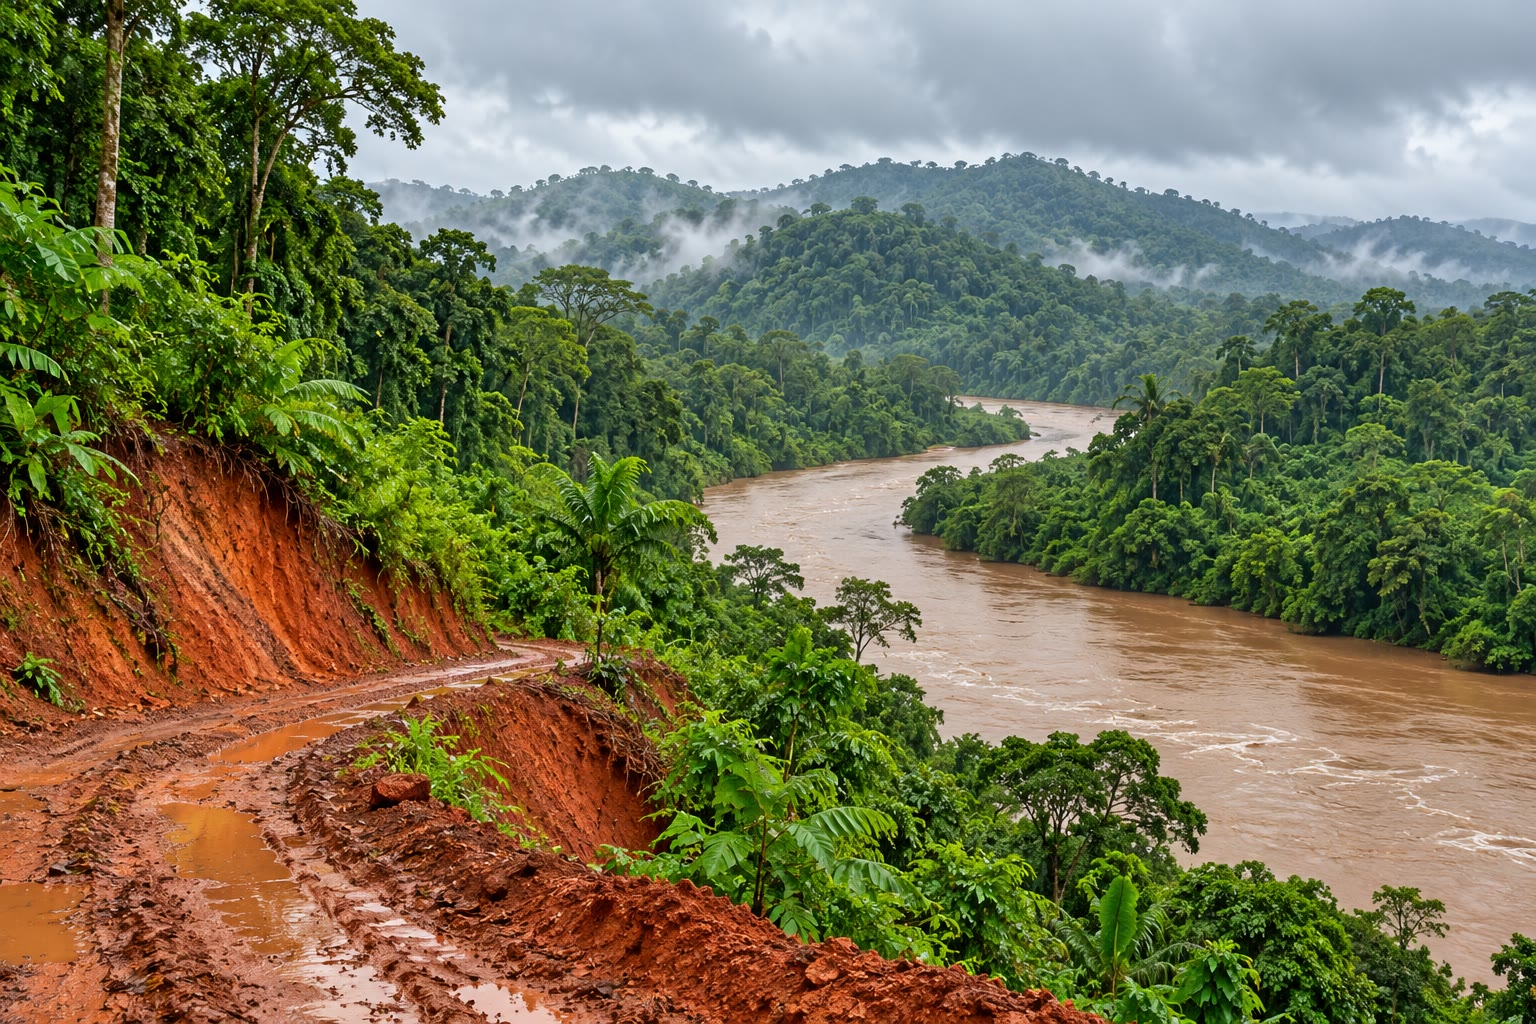
\includegraphics[width=0.66\linewidth]{images/book4/ai/b2-tropical-weathering.jpg}
\par\smallskip{\small जहाँ तापस्थापी सबसे कड़ी मेहनत करता है: एक गर्म, आर्द्र निचला मैदान, जहाँ वर्षा
गहराई तक अपक्षयित लाल मृदा पर गिरती है और नदी अपक्षय के उत्पादों को समुद्र तक ले जाती है
(AI से बनाया गया चित्रण)।}
\end{omfigure}

\section*{अभ्यास}\label{sec:b2:deep-time-climate:exercises}

अभ्यासों के आँकड़े, अन्यथा न कहा जाए तो: वायुमंडल में औद्योगिक-पूर्व कार्बन
\qty{591}{PgC} (\qty{278}{ppm}); $\qty{1}{Tmol}$ कार्बन $= \qty{0.012011}{PgC}$; सिलिकेट
अपक्षय $W_0 = \qty{0.138}{PgC.yr^{-1}}$; महासागर और कार्बोनेटों के बाद किसी अतिरिक्त का वायुवाहित
अंश $f = 0.08$; अपक्षय संवेदनशीलता $k_T = \qty{0.09}{K^{-1}}$; जलवायु संवेदनशीलता $S =
\qty{3}{K}$; कार्बन डाइऑक्साइड के दोगुनीकरण का प्रणोदन \qty{3.93}{W.m^{-2}}; $R =
\qty{8.314}{J.mol^{-1}.K^{-1}}$।
% ledger: ar6ch5:fig512, ipcc:erf-2xco2, derry24:fluxes, colbourn13:timescale, colbourn13:weathering, ipcc:ecs

\begin{exercise}[$\star$]\label{exo:b2:deep-time-climate:1}
औद्योगिक युग से पहले महासागर अपनी सतही परत में \qty{900}{PgC}, अपने मध्यवर्ती और गहरे जल में \num{37100},
घुले कार्बनिक कार्बन के रूप में 700 और अपने जीवित जीवों में 3 रखता था।
(क)~महासागर कितना कार्बन रखता था, और वायुमंडल का कितने गुना? (ख)~सतही भंडारों के
\qty{3.5e6}{Tmol} को पेटाग्राम कार्बन में बदलिए। (ग)~उसका कितना अंश वायु
में है?
\end{exercise}

\begin{exercise}[$\star$]\label{exo:b2:deep-time-climate:2}
\omterm{def:b2:deep-time-climate:carbon-cycle}{दीर्घकालिक कार्बन चक्र} के चित्र के प्रवाहों का उपयोग कीजिए, कायांतरी बहिर्गैसन को
\qty{3}{Tmol.yr^{-1}} लेकर। (क)~सतही भंडारों के निवेशों और निर्गमों का योग कीजिए।
(ख)~निवेशों का कितना अंश ज्वालामुखी, दरारें और \omterm{def:b2:metamorphic-facies:metamorphism}{कायांतरण} देते हैं? (ग)~निर्गमों का उपयोग करके सतही
भंडारों में कार्बन का निवास काल ज्ञात कीजिए।
\end{exercise}

\begin{exercise}[$\star$]\label{exo:b2:deep-time-climate:3}
(क)~कार्बन डाइऑक्साइड और जल द्वारा फ़ॉर्स्टेराइट, \ce{Mg2SiO4}, के मैग्नीशियम और बाइकार्बोनेट आयनों
तथा घुले सिलिका, \ce{SiO2}, में अपक्षय का समीकरण लिखिए और उसे संतुलित कीजिए। (ख)~मैग्नीशियम बाद में
कार्बोनेट के रूप में निक्षेपित होता है। शुद्ध अभिक्रिया लिखिए। (ग)~\qty{1}{PgC} को स्थायी रूप से हटाने के
लिए फ़ॉर्स्टेराइट के कितने द्रव्यमान का अपक्षय होना चाहिए? ($M(\ce{Mg2SiO4}) = \qty{140.7}{g.mol^{-1}}$।)
\end{exercise}

\begin{exercise}[$\star$]\label{exo:b2:deep-time-climate:4}
आयु के क्रम में, उनकी तिथियों के साथ, रखिए, और प्रत्येक के लिए बताइए कि पृथ्वी ग्रीनहाउस या
हिमगृह अवस्था में थी: आरंभिक इओसीन जलवायु इष्टतम; हिर्नेन्शियन हिमनदन; अंटार्कटिक हिमचादर का
आरंभ; ट्यूरोनियन; उत्तर पैलियोज़ोइक का सबसे बड़ा हिम-विस्तार; उत्तरी हिमचादरों की प्रमुख
बढ़तें; PETM।
\end{exercise}

\begin{exercise}[$\star\star$]\label{exo:b2:deep-time-climate:5}
(क)~जाँचिए कि \qty{63}{kJ.mol^{-1}} की सक्रियण ऊर्जा, \qty{288}{K} पर, $k_T =
\qty{0.09}{K^{-1}}$ देती है। (ख)~$k_T$ ज्ञात कीजिए, क्षेत्र-मान \qty{74}{kJ.mol^{-1}} के लिए। (ग)~प्रत्येक के
साथ, बहिर्गैसन के \qty{20}{\percent} बढ़ने पर स्थिर तापन ज्ञात कीजिए। (घ)~जलवायु
संवेदनशीलता (ग) में क्यों प्रवेश नहीं करती?
\end{exercise}

\begin{exercise}[$\star\star$]\label{exo:b2:deep-time-climate:6}
सटीक आरेनियस गुणक $\exp[-(E_{\text a}/R)(1/T - 1/T_0)]$ की तुलना $e^{k_T(T -
T_0)}$, $k_T = E_{\text a}/(RT_0^2)$, से कीजिए, $E_{\text a} = \qty{63}{kJ.mol^{-1}}$ और $T_0 =
\qty{288}{K}$ के लिए: (क)~$T = \qty{293}{K}$ पर; (ख)~$T = \qty{318}{K}$ पर। (ग)~दिखाइए कि सटीक
गुणक से सन्निकटन का अनुपात $\exp[E_{\text a}x^2/(RT_0^2(T_0 + x))]$ है, जहाँ $x = T - T_0$,
और वह तापन ज्ञात कीजिए जिस पर यह 1.1 तक पहुँचता है।
\end{exercise}

\begin{exercise}[$\star\star$]\label{exo:b2:deep-time-climate:7}
समतलित संकलन \qty{1444}{ppm} कार्बन डाइऑक्साइड देता है, \qty{419.5}{Ma} पर, और अपने अभिलेख के
अंत में \qty{276}{ppm}। (क)~उस गिरावट का प्रणोदन ज्ञात कीजिए। (ख)~उसकी तुलना चमकते सूर्य के
\qty{9}{W.m^{-2}} से कीजिए। (ग)~गिरावट की माध्य दर \unit{ppm} प्रति मिलियन वर्ष में ज्ञात कीजिए, और
उसकी तुलना समंजित प्रवृत्ति के \qty{3.4}{ppm} से कीजिए। वे भिन्न क्यों हो सकते हैं?
\end{exercise}
% ledger: data:b4-foster2017, foster17:co2

\begin{exercise}[$\star\star$]\label{exo:b2:deep-time-climate:8}
(क)~\num{3000} और \qty{7000}{PgC} को 3 और \qty{20}{kyr} पर फैलाइए: उत्सर्जन-दरों का कौन-सा परास
निकलता है? IPCC द्वारा उद्धृत 0.3 से \qty{1.5}{PgC.yr^{-1}} से तुलना कीजिए। (ख)~2010 में मानव उत्सर्जन
लगभग \qty{35}{Gt} कार्बन डाइऑक्साइड था। कार्बन में बदलिए और तुलना कीजिए। (ग)~कार्बन
डाइऑक्साइड 900 से \qty{2000}{ppm} तक बढ़ी। प्रणोदन, और $S =
\qty{3}{K}$ के साथ साम्य तापन, ज्ञात कीजिए, और PETM-पूर्व जलवायु पर \qty{5}{\celsius} के तापन से तुलना कीजिए।
\end{exercise}
% ledger: ar6ch5:petm-release, usgs:volcanic-co2, ar6ch5:petm

\begin{exercise}[$\star\star$]\label{exo:b2:deep-time-climate:9}
किसी पर्वत-पट्टी का उठना, स्थिर बहिर्गैसन पर, पृथ्वी की अपक्षयशीलता $W_0$ को 1.2 से गुणा कर देता है।
(क)~नया स्थिर तापमान-परिवर्तन ज्ञात कीजिए। (ख)~नई स्थिर कार्बन डाइऑक्साइड ज्ञात कीजिए,
\qty{278}{ppm} से आरंभ करके। (ग)~क्या नई स्थिर अवस्था में सिलिकेट अपक्षय की दर पुरानी से भिन्न है?
समझाइए।
\end{exercise}

\begin{exercise}[$\star\star\star$]\label{exo:b2:deep-time-climate:10}
(क)~अपवाह-गुणक के साथ तापस्थापी का e-गुना क्षय काल ज्ञात कीजिए, $k = 0.09 + 0.65\times0.045$।
(ख)~लाखों वर्षों में हिमचादरें और वनस्पति भी अनुक्रिया देती हैं; प्रति दोगुनीकरण \qty{8}{K} की
पृथ्वी-तंत्र संवेदनशीलता के साथ, $S$ के स्थान पर, $\tau$ ज्ञात कीजिए, $k_T$ लेकर। (ग)~दोनों परिवर्तन तापस्थापी को
किस ओर धकेलते हैं, और कौन-सी अनिश्चितता, $E_{\text a}$ या $S$, अधिक महत्त्व रखती है?
\end{exercise}

\begin{exercise}[$\star\star\star$]\label{exo:b2:deep-time-climate:11}
\qty{5000}{PgC} का एक उत्सर्जन (महासागर और कार्बोनेटों के बाद)। (क)~वायु की कार्बन डाइऑक्साइड, \unit{ppm} में,
और तापन ज्ञात कीजिए। (ख)~आरंभिक शुद्ध निष्कासन-दर $W - W_0$ ज्ञात कीजिए, और वह समय जो
स्पंद को उस दर पर लुप्त होने में लगेगा। (ग)~अतिरिक्त का \qty{90}{\percent} हटाने का रैखिकीकृत समय ज्ञात कीजिए।
(घ)~रैखिकीकरण के बिना समाकलित मॉडल \qty{340}{kyr} लेता है। अधिक लंबा क्यों?
\end{exercise}

\begin{exercise}[$\star\star\star$]\label{exo:b2:deep-time-climate:12}
(क)~मॉडल को उस स्थिर अवस्था के परितः रैखिकीकृत कीजिए जहाँ बहिर्गैसन $V$ और $C = C^*$ है, और दिखाइए कि
e-गुना क्षय काल $\tau' = A_0 (C^*/C_0)\ln 2/(f k S V)$ है। (ख)~बहिर्गैसन में \qty{20}{\percent} वृद्धि की
स्थिर अवस्था के लिए उसका मान निकालिए। (ग)~कार्बन डाइऑक्साइड से समृद्ध संसार में तापस्थापी तेज़ है या धीमा,
और क्यों?
\end{exercise}

\begin{problem}[{सप्ताहांत समस्या --- तापस्थापी कितना समय लेता है?}]\label{pb:b2:deep-time-climate:1}
यह समस्या मापे गए प्रवाहों से तापस्थापी का काल-नियतांक बनाती है। अभ्यासों के आँकड़ों का उपयोग कीजिए;
कटकों, \omterm{def:b2:oceanic-islands:stages}{महासागरीय द्वीपों}, चापों और दरारों पर बहिर्गैसन \num{1.3}, \num{1.3}, 4.5 और
\qty{4.2}{Tmol.yr^{-1}}; सिलिकेट अपक्षय 11 से \qty{12}{Tmol.yr^{-1}}; सक्रियण ऊर्जा
\qty{63}{kJ.mol^{-1}}, $T_0 = \qty{288}{K}$ पर; वायुमंडल का द्रव्यमान \qty{5.1e18}{kg}, वायु का माध्य मोलर
द्रव्यमान \qty{28.97}{g.mol^{-1}}। तीन सार्थक अंकों तक पूर्णांकित कीजिए।

\noindent\textbf{भाग I --- संतुलन।}
\begin{enumerate}
  \item ज्वालामुखीय और दरार बहिर्गैसन का योग कीजिए, \unit{Tmol.yr^{-1}} में और \unit{PgC.yr^{-1}} में।
  \item $W_0$ को उसके परास के मध्य में लीजिए; उसे \unit{PgC.yr^{-1}} में बदलिए।
  \item दोनों की तुलना कीजिए। यह तुलना \omterm{def:b2:deep-time-climate:carbon-cycle}{दीर्घकालिक कार्बन चक्र} के बारे में क्या सुझाती है?
  \item वायुमंडल में वायु के कितने मोल हैं? \qty{591}{PgC} कार्बन के कितने मोल हैं,
        और वह कौन-सा मिश्रण अनुपात है?
  \item बिल्कुल अपक्षय न होने पर, प्रश्न 1 का बहिर्गैसन सतही भंडारों में
        \qty{591}{PgC} जोड़ने में कितना समय लेगा?
  \item यदि उसका एक अंश $f = 0.08$ वायु में रहे, तो वायु की कार्बन
        डाइऑक्साइड किस गुणक से बढ़ेगी?
\end{enumerate}

\noindent\textbf{भाग II --- रैखिकीकरण।}
\begin{enumerate}[resume]
  \item सक्रियण ऊर्जा से $k_T$ ज्ञात कीजिए, और जाँचिए कि वह नीचे प्रयुक्त
        \qty{0.09}{K^{-1}} तक पूर्णांकित होता है।
  \item \qty{1}{K} के तापन के लिए अपक्षय किस गुणक से बढ़ता है?
  \item तापन $\Delta T$ किसी अतिरिक्त $M$ के लिए लिखिए, और $M = 0$ पर उसका अवकलज,
        \unit{K.PgC^{-1}} में।
  \item $W$ का अवकलज, $M$ के सापेक्ष, $M = 0$ पर ज्ञात कीजिए, \unit{yr^{-1}} में।
  \item दिखाइए कि उसका व्युत्क्रम \cref{prop:b2:deep-time-climate:thermostat} का
        काल-नियतांक $\tau$ है।
  \item $f$, $k$, $S$ और $W_0$ में से कौन-से बढ़ने पर तापस्थापी को तेज़ बनाते हैं?
\end{enumerate}

\noindent\textbf{भाग III --- काल-नियतांक।}
\begin{enumerate}[resume]
  \item $\tau$ का मान निकालिए।
  \item अपवाह-गुणक, $k = \qty{0.119}{K^{-1}}$, के साथ उसका मान निकालिए।
  \item $k_T$ और \qty{74}{kJ.mol^{-1}} की सक्रियण ऊर्जा के साथ उसका मान निकालिए।
  \item इन मानों की तुलना स्पष्ट महासागर वाले मॉडलों के \qty{200}{kyr} से \qty{1}{Myr} से कीजिए।
  \item कार्बन डाइऑक्साइड की सीनोज़ोइक गिरावट के \qty{50}{Myr} में कितने e-गुना क्षय काल समाते हैं?
        यह गिरावट के दौरान कार्बन चक्र की अवस्था के बारे में क्या बताता है?
  \item प्रति मिलियन वर्ष \qty{16}{ppm} की दर से, एक $\tau$ में कार्बन डाइऑक्साइड कितनी बदलती है?
\end{enumerate}

\noindent\textbf{भाग IV --- PETM के आकार का उत्सर्जन।}
\begin{enumerate}[resume]
  \item \qty{5000}{PgC} उत्सर्जित होता है; महासागर और कार्बोनेटों के कार्य कर लेने के बाद कितना
        वायु में रहता है, और \unit{ppm} में कार्बन डाइऑक्साइड क्या है?
  \item उस क्षण तापन ज्ञात कीजिए।
  \item अपक्षय-दर कितनी बढ़ती है, \unit{PgC.yr^{-1}} में और प्रतिशत में?
  \item रैखिकीकृत नियम से, अतिरिक्त का \qty{90}{\percent} जाने में कितना समय लगेगा?
  \item PETM का कार्बोनेट लगभग \qty{100}{kyr} में पुनर्प्राप्त हुआ। दो कारण बताइए कि वास्तविक
        पृथ्वी इस मॉडल से तेज़ क्यों रही होगी।
  \item सारांश में: इस मॉडल में \omterm{def:b2:deep-time-climate:thermostat}{सिलिकेट-अपक्षय तापस्थापी} का e-गुना क्षय काल क्या है?
\end{enumerate}
\end{problem}
% ledger: derry24:fluxes, colbourn13:weathering, colbourn13:timescale, ar6ch5:fig512, ar6ch5:petm, ar6ch5:cenozoic-co2, ipcc:ecs, earth:Matm, earth:Mmol
